\documentclass[xcolor={usenames,dvipsnames,svgnames,table}]{beamer}

\usepackage[english,russian]{babel}
\usepackage[T2A,T1]{fontenc}

\usetheme[usetitleprogressbar]{m}

\usefonttheme{professionalfonts}

\usepackage{amsmath}

\usepackage{tikz}
\usetikzlibrary{positioning}
\usetikzlibrary{decorations.text}
\usetikzlibrary{decorations.pathmorphing}


\usepackage{standalone}
\usepackage{subfiles}

\usepackage{graphicx}
\usepackage{hyperref}

\usepackage{tabularx}
\usepackage{array}
\usepackage{multirow}

\usepackage{gensymb}

\usepackage{subfigure}
\usepackage{gnuplottex}

\usepackage{python}

\setbeamertemplate{caption}{\raggedright\tiny\insertcaption\par}

\newcommand{\disser}{Численное решение трёхмерных задач\\
                     разрушения инженерных конструкций\\
                     при разных режимах нагружения}

\newcommand{\twofigscommon}[7]{
    \begin{figure}[#7]
        \centering
        \subcaptionbox{#4}{\includegraphics[width=0.45\linewidth]{#3}}
        \subcaptionbox{#6}{\includegraphics[width=0.45\linewidth]{#5}}
        \caption{#2}
        \label{#1}
    \end{figure}
}

\newcommand{\twofigs}[6]{ \twofigscommon{#1}{#2}{#3}{#4}{#5}{#6}{ht} }

\newcommand{\twofigsH}[6]{ \twofigscommon{#1}{#2}{#3}{#4}{#5}{#6}{h!} }
\newcommand{\twofigsT}[6]{ \twofigscommon{#1}{#2}{#3}{#4}{#5}{#6}{t!} }

\newcommand{\threefigscommon}[9]{
    \begin{figure}[#9]
        \centering
        \subcaptionbox{#4}{\includegraphics[width=0.30\linewidth]{#3}}
        \subcaptionbox{#6}{\includegraphics[width=0.30\linewidth]{#5}}
        \subcaptionbox{#8}{\includegraphics[width=0.30\linewidth]{#7}}
        \caption{#2}
        \label{#1}
    \end{figure}
}

\newcommand{\threefigs}[8]{ \threefigscommon{#1}{#2}{#3}{#4}{#5}{#6}{#7}{#8}{ht} }
\newcommand{\threefigsH}[8]{ \threefigscommon{#1}{#2}{#3}{#4}{#5}{#6}{#7}{#8}{h!} }

\newcommand{\figsub}[4]{
    \begin{figure}[ht]
        \centering
        \begin{subfigure}{0.45\linewidth}
            \centering
            \includegraphics[width=\textwidth]{#3}
            \caption{#4}
        \end{subfigure}
        \caption{#2}
        \label{#1}
    \end{figure}
}

\newcommand{\twofigsminipage}[6]{
    \begin{figure}[ht]
        \begin{minipage}[b]{0.45\linewidth}
            \centering
            \includegraphics[width=\textwidth]{#1}
            \caption{#3}
            \label{#2}
        \end{minipage}
        \begin{minipage}[b]{0.45\linewidth}
            \centering
            \includegraphics[width=\textwidth]{#4}
            \caption{#6}
            \label{#5}
        \end{minipage}
    \end{figure}
}

\newcommand{\figminipage}[3]{
    \begin{figure}[ht]
        \begin{minipage}[b]{0.45\linewidth}
            \centering
            \includegraphics[width=\textwidth]{#1}
            \caption{#3}
            \label{#2}
        \end{minipage}
    \end{figure}
}

\newcommand{\figcommon}[5]{
    \begin{figure}[#5]
        \centering
        \includegraphics[width=#4]{#2}
        \caption{#3}
        \label{#1}
    \end{figure}
}

\newcommand{\fig}[3]{
    \figcommon{#1}{#2}{#3}{0.45\linewidth}{ht}
}

\newcommand{\figsmall}[3]{
    \figcommon{#1}{#2}{#3}{0.35\linewidth}{ht}
}

\newcommand{\figsmallH}[3]{
    \figcommon{#1}{#2}{#3}{0.35\linewidth}{h!}
}

\newcommand{\figH}[3]{
    \figcommon{#1}{#2}{#3}{0.45\linewidth}{h!}
}

\newcommand{\figfull}[3]{
    \figcommon{#1}{#2}{#3}{0.80\linewidth}{ht}
}

\newcommand{\figfullH}[3]{
    \figcommon{#1}{#2}{#3}{0.80\linewidth}{h!}
}

\newcommand{\ctodo}{\todo[color=red]}
\newcommand{\ntodo}{\todo[color=blue!40]}
\newcommand{\rtodo}{\todo}

\newcolumntype{L}[1]{>{\raggedright\let\newline\\\arraybackslash\hspace{0pt}}m{#1}}
\newcolumntype{C}[1]{>{\centering\let\newline\\\arraybackslash\hspace{0pt}}m{#1}}
\newcolumntype{R}[1]{>{\raggedleft\let\newline\\\arraybackslash\hspace{0pt}}m{#1}}

\newcommand\abs[1]{\left|#1\right|}

\newcommand{\PD}[2]{\frac{\partial{#1}}{\partial{#2}}}
\newcommand{\TD}[2]{\frac{d#1}{d#2}}

\newcommand{\PDx}[1]{\PD{#1}{x}}
\newcommand{\PDy}[1]{\PD{#1}{y}}
\newcommand{\PDz}[1]{\PD{#1}{z}}
\newcommand{\PDt}[1]{\PD{#1}{t}}

\newcommand{\TDt}[1]{\TD{#1}{t}}

\newcommand{\Sxx}{\sigma_{xx}}
\newcommand{\Sxy}{\sigma_{xy}}
\newcommand{\Sxz}{\sigma_{xz}}
\newcommand{\Syy}{\sigma_{yy}}
\newcommand{\Syz}{\sigma_{yz}}
\newcommand{\Szz}{\sigma_{zz}}

\newcommand{\Bad}[1]{\textbf{\color{OrangeRed}#1}}
\newcommand{\Good}[1]{\textbf{\color{OliveGreen}#1}}

\newcommand\Wider[2][3em]{
\makebox[\linewidth][c]{
    \begin{minipage}{\dimexpr\textwidth+#1\relax}
    \raggedright#2
    \end{minipage}
    }
}

\title{Численное решение трёхмерных задач\\разрушения инженерных конструкций\\при разных режимах нагружения}
\author{Алексей Сергеевич Ермаков\newline\tiny{Научный руководитель: д.ф.-м.н., чл.-корр. РАН, проф. И.Б. Петров}}
\institute{Московский физико-технический институт}
\date{Москва, 2015}
\titlegraphic{
\includegraphics[width=.25\textwidth]{eps/mipt.eps}}

\begin{document}
\setbeamerfont{page number in head/foot}{size=\huge}

\frame[plain]{\titlepage}

\frame{\frametitle{Уравнения МДТТ}
    \begin{eqnarray*}
        \rho\dot{v}_i=\nabla_j\sigma_{ij}+f_i & \textnormal{(уравнения движения)} \\
        \dot\sigma_{ij}=q_{ijkl}\dot{\varepsilon}_{kl}+F_{ij} & \textnormal{(реологические соотношения)} \\
        \dot{\varepsilon}_{ij}=\frac{1}{2}(\nabla_j v_i+\nabla_i v_j)
    \end{eqnarray*}

    \begin{tabular}[h!]{lcl}
        $\rho$ &~--- & плотность \\
        $\sigma_{ij}$ &~--- & тензор напряжений \\
        $f_i$ &~--- & массовые силы, действующие на~единицу объёма \\
        $q_{ijkl}$ &~--- & тензор, определяемый реологией среды \\
        $\dot\varepsilon_{ij}$ &~--- & тензор скоростей деформаций \\
        $F_{ij}$ &~--- & добавочная правая часть \\
        $\nabla_j$ &~--- & ковариантная производная по~$j$-й координате
    \end{tabular}
}

\frame{\frametitle{Линейно-упругое анизотропное приближение}
    \vspace{-2.5em}
    \begin{small}
    \begin{eqnarray*}
    \frac{\partial\vec{u}}{\partial{t}}+\mathbf{A}_x\frac{\partial\vec{u}}{\partial{x}}
                                        +\mathbf{A}_y\frac{\partial\vec{u}}{\partial{y}}
                                        +\mathbf{A}_z\frac{\partial\vec{u}}{\partial{z}}
                                        =F(x,y,z,t)
    \\
    \vec{u}=\{v_x,v_y,v_z,\sigma_{xx},\sigma_{xy},\sigma_{xz},\sigma_{yy},\sigma_{yz},\sigma_{zz}\}^T
    \end{eqnarray*}
    \begin{eqnarray*}
    2q_{ijkl} & = & c_{ik}\delta_{ij}\delta_{kl} + \sum_{m=1}^{3}\sum_{n=1}^{3}c_{m+3,n+3}\abs{\varepsilon_{mij}}\abs{\varepsilon_{nkl}} + {} \\
                & + & \sum_{m=1}^{3}c_{i,m+3}\delta_{ij}\abs{\varepsilon_{mkl}} + \sum_{m=1}^{3}c_{m+3,k}\abs{\varepsilon_{mij}}\delta_{kl}
    \end{eqnarray*}

    \begin{minipage}[h!]{0.45\textwidth}
    \begin{align*}
        c_{ik} =
        \left( \begin{array}{cccccccccccc}
        c_{11} & c_{12} & c_{13} & c_{14} & c_{15} & c_{16} \\
        c_{12} & c_{22} & c_{23} & c_{24} & c_{25} & c_{26} \\
        c_{13} & c_{23} & c_{33} & c_{34} & c_{35} & c_{36} \\
        c_{14} & c_{24} & c_{34} & c_{44} & c_{45} & c_{46} \\
        c_{15} & c_{25} & c_{35} & c_{45} & c_{55} & c_{56} \\
        c_{16} & c_{26} & c_{36} & c_{46} & c_{56} & c_{66}
        \end{array} \right)
    \end{align*}
    \end{minipage}
    \begin{minipage}[h!]{0.3\textwidth}
        \begin{tabular}[h!]{p{0.3cm} p{0.4cm} l}
        $\delta_{ij}$       &~--- & символ \\
                            &     & Кронекера \\
        $\varepsilon_{ijk}$ &~--- & символ \\
                            &     & Леви-Чевиты
        \end{tabular}
    \end{minipage}
    \end{small}
}

\frame{\frametitle{Критерии разрушения}
    \begin{minipage}[h!]{0.50\textwidth}
        \begin{itemize}
            \item Критерий наибольших главных напряжений
            \item Критерий Друкера-Прагера
            \item Критерий Хашина
            \item Критерий Пака
            \item Критерий Цая-Хилла
            \item Критерий Цая-Ву
            \item Адгезионная прочность
        \end{itemize}
    \end{minipage}
    \vrule
    \begin{minipage}[h!]{0.45\textwidth}
        \begin{itemize}
            \item Однобереговая модель трещин
            \item Дискретное скалярное разрушение
        \end{itemize}
    \end{minipage}
}

\frame{\frametitle{Случай больших деформаций}
    \Wider[2em]{
    \begin{minipage}[h!]{0.20\textwidth}
        \tiny
        \begin{align*}
            \frac{d\rho}{dt} &= -\rho \PD{u_\alpha}{x_\alpha} \\
            \frac{du_\alpha}{dt} &= \frac{1}{\rho}\PD{\sigma_{\alpha\beta}}{x_\beta} \\
            \frac{de}{dt} &= \frac{1}{\rho}\sigma_{\alpha\beta}\varepsilon_{\alpha\beta} \\
            R_{\alpha\beta} &= \frac{1}{2}\left( \PD{u_\alpha}{x_\beta} - \PD{u_\beta}{x_\alpha}\right) \\
            \varepsilon_{\alpha\beta} &= \frac{1}{2}\left( \PD{u_\alpha}{x_\beta} + \PD{u_\beta}{x_\alpha}\right) \\
            \frac{dS_{\alpha\beta}}{dt} &= 2\mu \left( \varepsilon_{\alpha\beta}-\frac{1}{3}\delta_{\alpha\beta}\varepsilon_{\alpha\beta} \right) + \\
                                        &+  S_{\alpha\gamma}R_{\beta\gamma}+S_{\gamma\beta}R_{\alpha\gamma}- \\
                                        &-  \theta(s)(S_{\alpha\beta}\varepsilon_{\alpha\beta})S_{\alpha\beta} \\
             P(\rho,e) &= \frac{K}{n}\left( \left( \frac{\rho}{\rho_0} \right)^n -1  \right)
        \end{align*}
    \end{minipage}
    \qquad{\color{black}\vrule}\qquad
    \begin{minipage}[h!]{0.35\textwidth}
        \tiny
        \begin{align*}
            \rho &- \textnormal{плотность} \\
            u_\alpha &- \textnormal{скорость} \\
            \sigma_{\alpha\beta} &- \textnormal{тензор напряжений} \\
            S_{\alpha\beta} &- \textnormal{девиатор тензора напряжений} \\
            P &- \textnormal{давление} \\
            e &- \textnormal{внутренняя энергия} \\
            K,n &- \textnormal{константы}
        \end{align*}
        \[
            \theta(s)=\left\{\begin{aligned}
                0, & при s<2K^2 \\
                0, & при s=2K^2, S_{\alpha\beta}\varepsilon_{\alpha\beta} \leq 0\\
                \frac{\mu}{K^2}, & при s=2K^2, S_{\alpha\beta}\varepsilon_{\alpha\beta} > 0
            \end{aligned}\right.
        \]
    \end{minipage}
    }
}

\frame{\frametitle{Сеточно-характеристический метод}
    \[
        \frac{\partial\vec{u}}{\partial{t}}+\mathbf{A}_x\frac{\partial\vec{u}}{\partial{x}}
                                            +\mathbf{A}_y\frac{\partial\vec{u}}{\partial{y}}
                                            +\mathbf{A}_z\frac{\partial\vec{u}}{\partial{z}}
                                            =F(x,y,z,t)
    \]
    \begin{minipage}[h!]{0.4\textwidth}
        \begin{eqnarray*}
            \frac{\partial}{\partial t}\vec u+\mathbf{A}_x \frac{\partial}{\partial x}\vec u
            = 0 \\
            \frac{\partial}{\partial t}\vec u+\mathbf{A}_y \frac{\partial}{\partial y}\vec u
            = 0 \\
            \frac{\partial}{\partial t}\vec u+\mathbf{A}_z \frac{\partial}{\partial z}\vec u
            = 0 \\
            \frac{\partial}{\partial t}\vec u = \vec f
        \end{eqnarray*}
    \end{minipage}
    \qquad{\color{black}\vrule}\qquad
    \begin{minipage}[h!]{0.4\textwidth}
        \begin{eqnarray*}
            \mathbf{A}=\mathbf{\Omega^{-1}}\mathbf{\Lambda}\mathbf{\Omega} \\
            \vec \omega = \mathbf{\Omega} \cdot \vec u \\
            \frac{\partial \omega_i}{\partial t}+\lambda_i \frac{\partial \omega_i}{\partial x_j} = 0
        \end{eqnarray*}
        \tiny
        \begin{figure}[h]
            \begin{center}
                \tikzset{every picture/.style={scale=0.33}}
                \subfile{tikz/gcm}
            \end{center}
        \end{figure}
    \end{minipage}
}

\frame{\frametitle{Метод сглаженных частиц (SPH)}
    \begin{minipage}[h!]{0.57\textwidth}
        \begin{itemize}
            \item Бессеточный метод
            \item Аппроксимация при помощи ядра сглаживания
            \item Искусственная вязкость для подавления нефизичных осцилляций
            \item Использования аналитического решения задачи Римана
            \item Гибридный метод
        \end{itemize}
    \end{minipage}
    \begin{minipage}[h!]{0.35\textwidth}
        \begin{figure}[h]
            \begin{center}
                \tikzset{every picture/.style={scale=0.75}}
                \subfile{tikz/sph}
            \end{center}
        \end{figure}
    \end{minipage}
    \begin{eqnarray*}
        \bar a(x)=\int_R \left[\frac{a(x')}{\rho(x')}\right]\omega(x'-x,h)\rho(x')dx' \\
        \omega(x,h) \xrightarrow[h \to 0]{} \delta(x)
    \end{eqnarray*}
}

\frame{\frametitle{Комбинированный метод (SPGCM)}
    \begin{minipage}[h!]{0.85\textwidth}
        Особенности:
        \begin{itemize}
            \item Объединение двух методов: SPH и GCM
            \item Решение задач с~большими деформациями
            \item Корректный учёт контактных условий
            \item Получение полной волновой картины
        \end{itemize}

        Решённые проблемы:
        \begin{itemize}
            \item «Склеивание» методов
            \item Реализация параллельного алгоритма
        \end{itemize}
    \end{minipage}
    \begin{minipage}[h!]{0.13\textwidth}
        \begin{center}
            \tikzset{every picture/.style={scale=0.9,rotate=-90}}
            \subfile{tikz/spgcm}
        \end{center}
    \end{minipage}
}

\begin{python}
#!/bin/env python2
# -*- coding: utf-8 -*-
for i in range(10):
    print('\\frame{\\frametitle{Верификация SPGCM: распад разрыва}')
    print('\\includegraphics[width=\\textwidth]{png/spgcm/OneStep-normal/pics/1D-V.X-%d-transparent.png}}''' % i)
    print('\\addtocounter{framenumber}{-1}')
\end{python}

\addtocounter{framenumber}{+1}
\begin{python}
#!/bin/env python2
# -*- coding: utf-8 -*-
for i in range(10):
    print('\\frame{\\frametitle{Верификация SPGCM: синусоидальное возмущение}')
    print('\\includegraphics[width=\\textwidth]{png/spgcm/Sine-normal/pics/1D-V.X-%d-transparent.png}}''' % i)
    print('\\addtocounter{framenumber}{-1}')
\end{python}

\addtocounter{framenumber}{+1}

\frame{\frametitle{Падение самолёта на~крышу здания}
    \Wider{
        \begin{minipage}[h!]{0.3\textwidth}
            \begin{center}
                \begin{figure}[h]
                    \tikzset{every picture/.style={scale=0.2}}
                    \subfile{tikz/air_nuke}
                \end{figure}
            \end{center}
            \hrule
            \begin{center}
                \begin{figure}[h]
                    \tikzset{every picture/.style={scale=0.3}}
                    \subfile{tikz/air_nuke_engines}
                \end{figure}
            \end{center}
        \end{minipage}
        \qquad\vrule\qquad
        \begin{minipage}[h!]{0.4\textwidth}
            \small
            \begin{tabular}{l | l}
                \textbf{Длина фюзеляжа} & 10~м \\
                \textbf{Толщина преграды} & 1~м \\
                \textbf{Радиус оболочки} & 10~м \\
                \textbf{Материал фюзеляжа} & дюралюминий \\
                \textbf{Материал преграды} & бетон \\
                \textbf{Скорость подхода} & 250~м/c и 400~м/c \\
            \end{tabular}
        \end{minipage}
    }
}

\begin{python}
#!/bin/env python2
# -*- coding: utf-8 -*-
for n in [0, 6, 12, 18, 24, 30, 36, 42, 48, 54, 60, 69]:
    print('\\frame{\\frametitle{Падение самолёта на~крышу здания: фюзеляж}')
    print('\\begin{center}')
    print('\\includegraphics[width=\\textwidth]{png/air-nuke/2D-VELOCITY-ABS-%d-transparent.png}' % n)
    print('\\end{center}}')
    print('\\addtocounter{framenumber}{-1}')
\end{python}

\addtocounter{framenumber}{+1}

\begin{python}
#!/bin/env python2
# -*- coding: utf-8 -*-
for n in [0, 45, 90, 135, 180, 225, 270, 315, 360, 399]:
    print('\\frame{\\frametitle{Падение самолёта на~крышу здания: двигатели}')
    print('\\begin{center}')
    print('\\includegraphics[width=\\textwidth]{png/air-nuke-engines/2D-VELOCITY-ABS-%d-transparent.png}' % n)
    print('\\end{center}}')
    print('\\addtocounter{framenumber}{-1}')
\end{python}

\addtocounter{framenumber}{+1}
\frame{\frametitle{Столкновение спутника с~микрометеоритом}
    \Wider{
        \begin{minipage}[h!]{0.25\textwidth}
            \begin{center}
                \begin{figure}[h]
                    \tikzset{every picture/.style={scale=0.12}}
                    \subfile{tikz/satellite}
                \end{figure}
            \end{center}
        \end{minipage}
        \qquad\vrule\qquad
        \begin{minipage}[h!]{0.4\textwidth}
            \small
            \begin{tabular}{l | l}
                \textbf{Диаметр внешней оболочки} & 5~м \\
                \textbf{Толщина внешней оболочки} & 0.4~м \\
                \textbf{Диаметр внутренней оболочки} & 1.7~м \\
                \textbf{Толщина внутренней оболочки} & 0.2~м \\
                \textbf{Диаметр микрометеорита} & 0.3~м \\
                \textbf{Материал корпуса} & пластик \\
                \textbf{Материал микрометеорита} & железо \\
                \textbf{Скорость подхода} & 3200~м/c \\
            \end{tabular}
        \end{minipage}
    }
}

\begin{python}
#!/bin/env python2
# -*- coding: utf-8 -*-
for n in [0, 450, 900, 1350, 1800, 2250, 2700, 3150, 3600, 3999]:
    print('\\frame{\\frametitle{Столкновение спутника с~микрометеоритом}')
    print('\\begin{center}')
    print('\\includegraphics[width=0.9\\textwidth]{png/satellite/2D-VELOCITY-ABS-%d-transparent.png}' % n)
    print('\\end{center}}')
    print('\\addtocounter{framenumber}{-1}')
\end{python}

\addtocounter{framenumber}{+1}

\frame{\frametitle{Решение задачи о~пробивании}
    \begin{tabular}[h]{c|c|c}
        Форма ударника & Угол к~нормали & Скорость на~подходе \\ \hline
        Шар            & 0\degree       & 925~м/с \\
        Шар            & 30\degree      & 1200~м/с
    \end{tabular}
    \begin{figure}[ht]
        \begin{minipage}[b]{0.70\linewidth}
            \centering
            \includegraphics[width=\textwidth]{png/spgcm/sphere-test-transparent.png}
        \end{minipage}
    \end{figure}
}

\begin{frame}[fragile]
    \frametitle{Решение задачи о~пробивании, шар, 30\degree}
    \begin{center}
        \tiny
        \begin{gnuplot}
            set datafile separator ","
            set terminal epslatex color size 10cm, 7cm 8
            set grid ytics xtics
            set grid
            set xlabel "t, мкс"
            set ylabel "$v_x$, м/с"
            set xrange [0:30]
            set yrange [0:1200]
            plot "csv/angled-sphere-spgcm.csv" title "SPGCM", \
                "csv/angled-sphere-dyna.csv" title "LS-DYNA" with points pointtype 7
        \end{gnuplot}
    \end{center}
\end{frame}

\begin{frame}[fragile]
    \frametitle{Решение задачи о~пробивании, шар, 0\degree}
    \begin{center}
        \tiny
        \begin{gnuplot}
            set datafile separator ","
            set terminal epslatex color size 10cm, 7cm 8
            set grid ytics xtics
            set grid
            set xlabel "t, мкс"
            set ylabel "$v_x$, м/с"
            set xrange [0:30]
            set yrange [0:1200]
            plot "csv/normal-sphere-spgcm.csv" title "SPGCM", \
                "csv/normal-sphere-dyna.csv" title "LS-DYNA" with points pointtype 7
        \end{gnuplot}
    \end{center}
\end{frame}

\frame{\frametitle{Трёхмерный метод маркеров}
    \Wider{
        \begin{itemize}
            \item Комбинация сеточно-характеристического метода и метода маркеров
            \item Использует одновременно подвижную и неподвижную сетки
            \item Позволяет считать задачи с~большими деформациями
            \item Обладает фиксированным шагом по~времени
        \end{itemize}
        \centering\includegraphics[width=0.65\textwidth]{png/markers/mesh-transparent.png}
    }
}

\frame{\frametitle{Трёхмерный метод маркеров: решенные проблемы}
    \begin{minipage}[h!]{0.55\textwidth}
        \begin{itemize}
            \item Реконструкция границы
            \item Уточнение границ
            \item Вычисление нормалей
            \item Экстраполяция значений
        \end{itemize}
        \vspace{3.5em}
        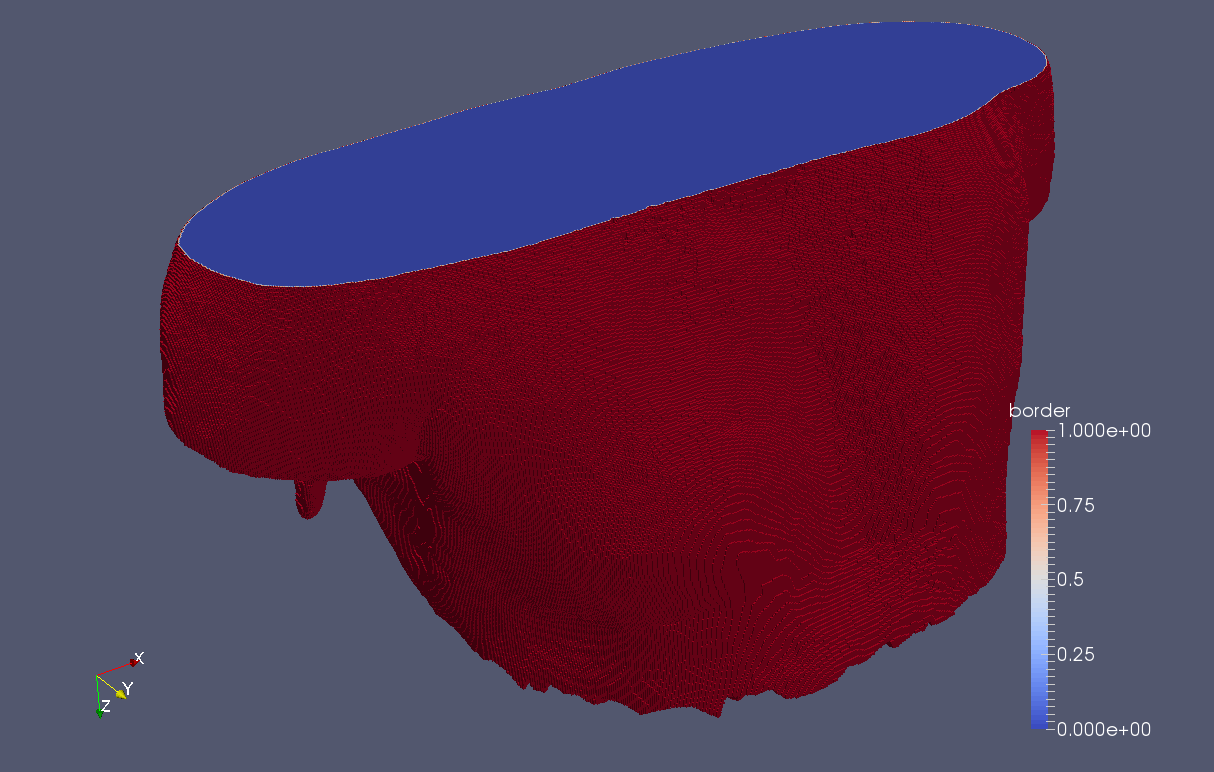
\includegraphics[width=0.8\textwidth]{png/markers/body.png}
    \end{minipage}
    \begin{minipage}[h!]{0.4\textwidth}
        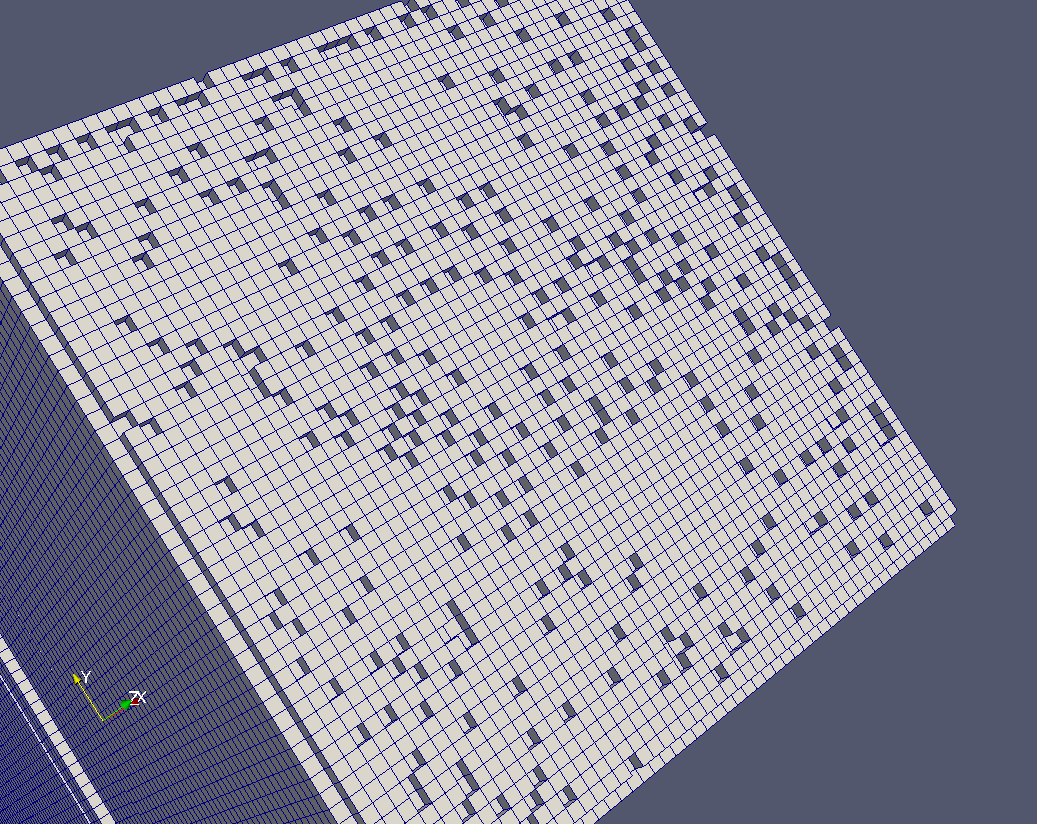
\includegraphics[width=\textwidth]{png/markers/before-refinement.png}
        \newline
        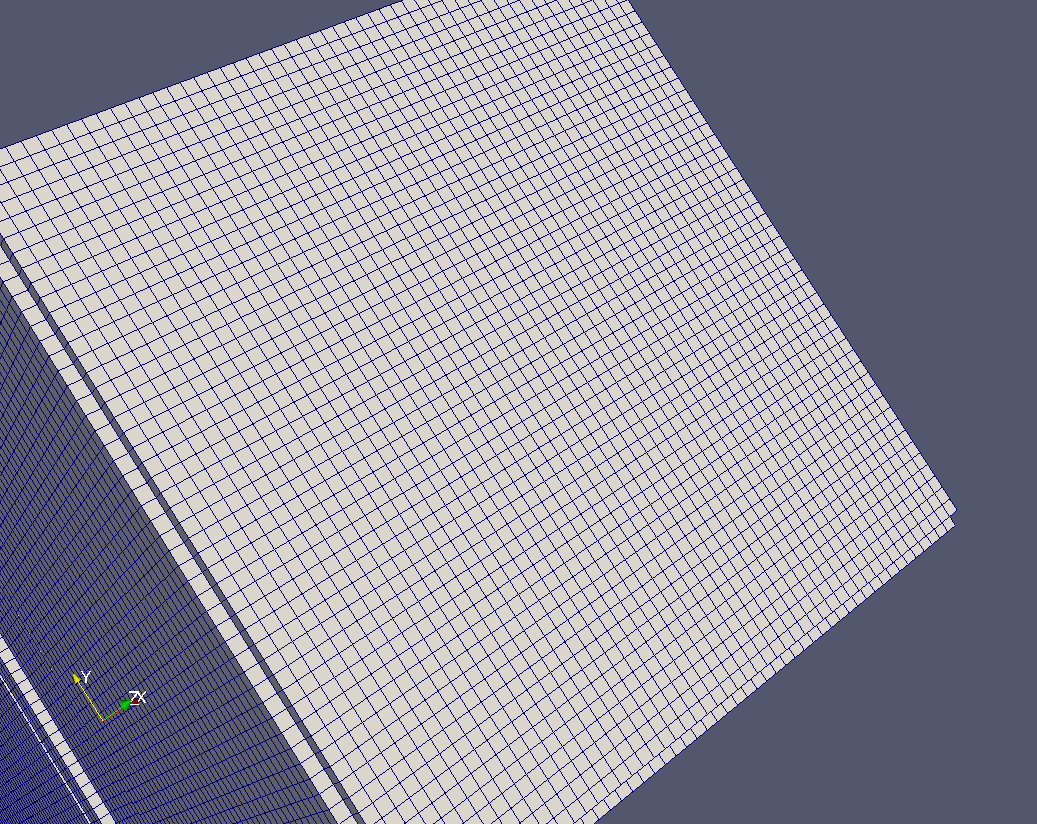
\includegraphics[width=\textwidth]{png/markers/after-refinement.png}
    \end{minipage}
}

\begin{frame}
    \frametitle{Трёхмерный метод маркеров: пример деформаций}
    \begin{center}
        \begin{minipage}[h]{0.47\textwidth}
            \begin{figure}[h]
                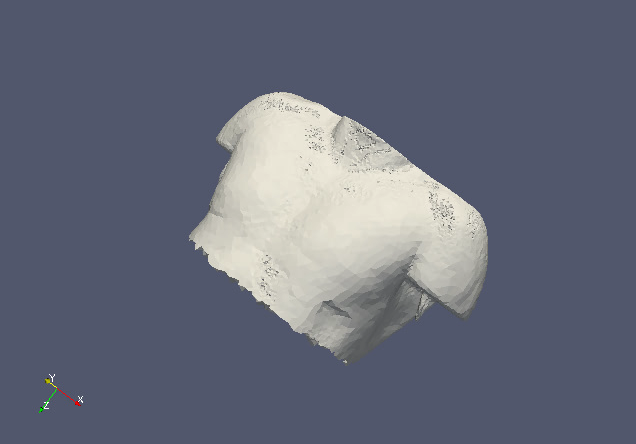
\includegraphics[width=\textwidth]{png/corpse/image1.png}
            \end{figure}
        \end{minipage}
        \begin{minipage}[h]{0.47\textwidth}
            \begin{figure}[h]
                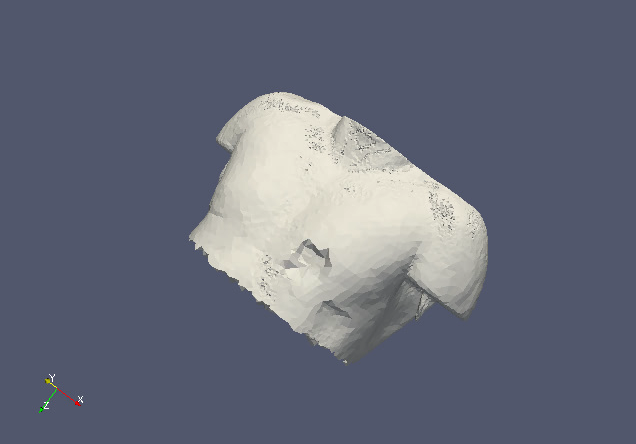
\includegraphics[width=\textwidth]{png/corpse/image2.png}
            \end{figure}
        \end{minipage}
        \begin{minipage}[h]{0.47\textwidth}
            \begin{figure}[h]
                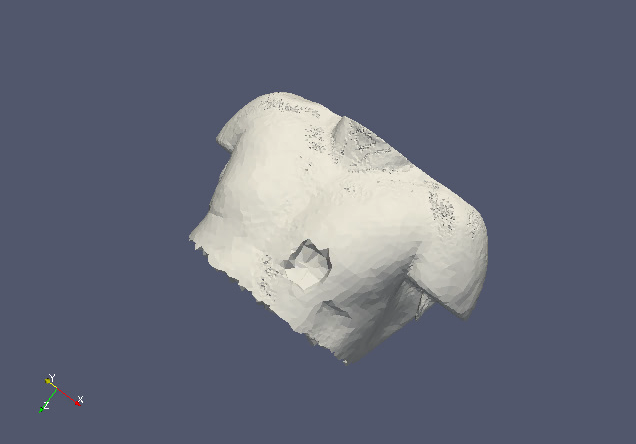
\includegraphics[width=\textwidth]{png/corpse/image3.png}
            \end{figure}
        \end{minipage}
        \begin{minipage}[h]{0.47\textwidth}
            \begin{figure}[h]
                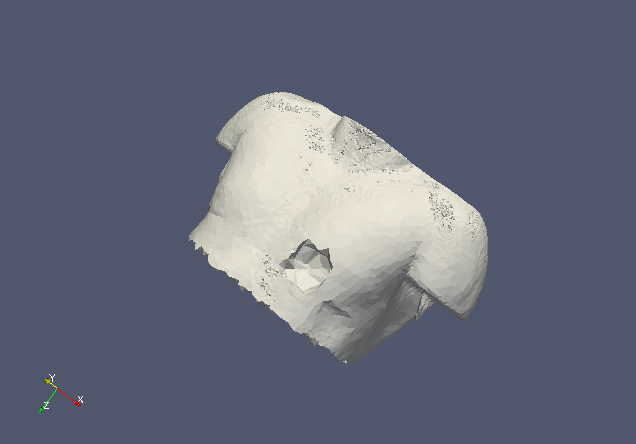
\includegraphics[width=\textwidth]{png/corpse/image4.png}
            \end{figure}
        \end{minipage}
    \end{center}
\end{frame}

\frame{\frametitle{Разрушение стекла под действием лазерного излучения}
    \Wider{
        \begin{minipage}[h!]{0.42\textwidth}
            \begin{center}
                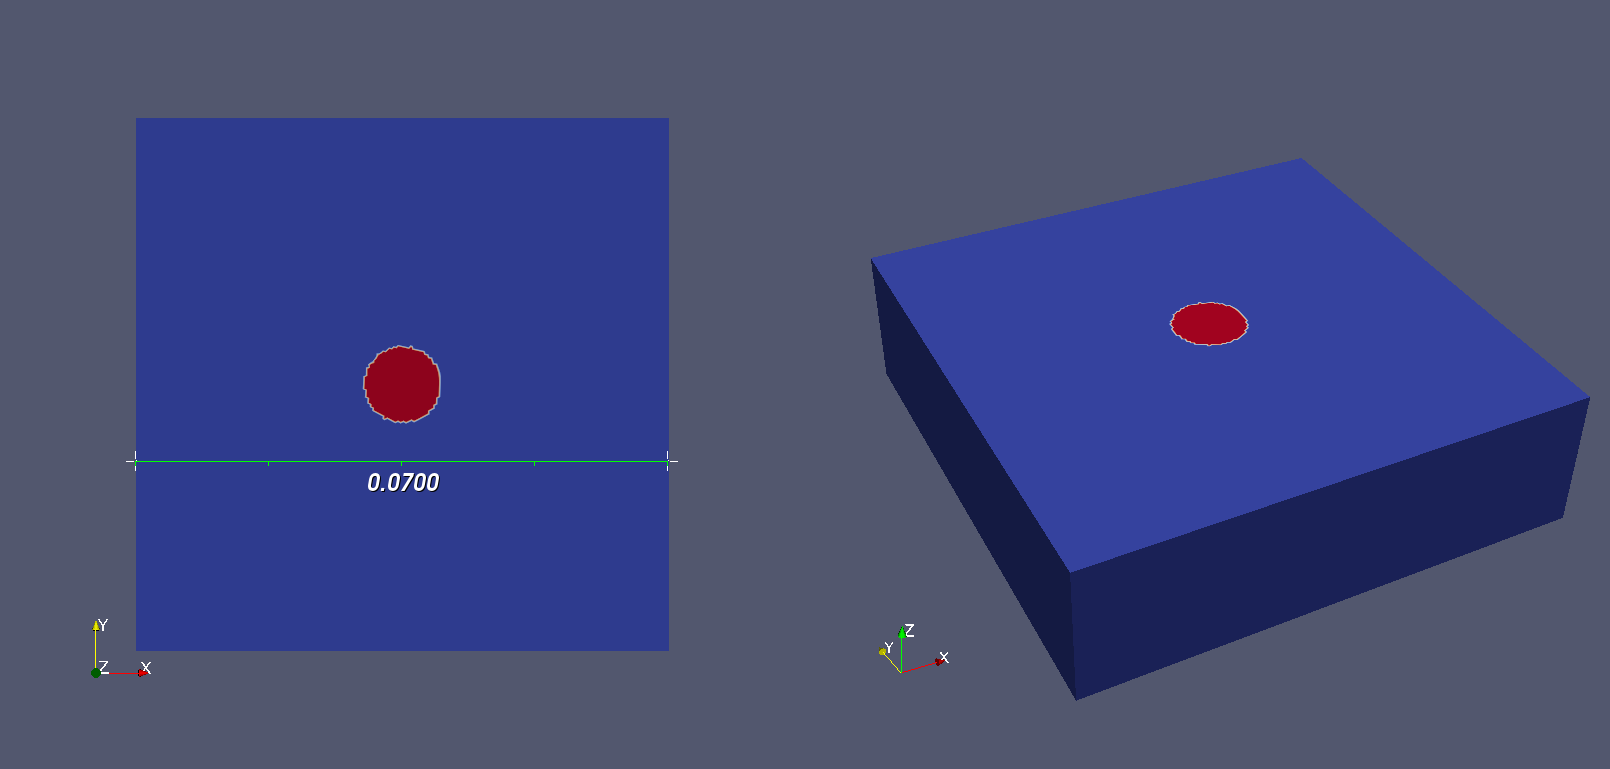
\includegraphics[width=\textwidth]{png/glass/glass-laser-pressure.png}
                \begin{table}[ht]
                    \centering
                    \footnotesize
                    \begin{tabular}{l | l}
                        \textbf{Длительность импульса} & 5~мкс \\
                        \textbf{Давление} & 8 ГПа \\
                        \textbf{Радиус области давления} & 5~мм \\
                    \end{tabular}
                \end{table}
            \end{center}
        \end{minipage}
        \quad\vrule\quad
        \begin{minipage}[h!]{0.4\textwidth}
            \small
            \begin{tabular}{l | l}
                \textbf{Размеры} & 70x70x20~мм \\
                \textbf{Тип материала} & Изотропный \\
                \textbf{Коэффициент Ламэ $\lambda$} & 22.5 ГПа \\
                \textbf{Коэффициент Ламэ $\mu$} & 28.7 ГПа \\
                \textbf{Плотность} & 2500 $\textnormal{кг}/\textnormal{см}^3$ \\
                \textbf{Предел прочности} & 1.5 ГПа \\
            \end{tabular}
        \end{minipage}
    }
}

\begin{python}
#!/bin/env python2
# -*- coding: utf-8 -*-
for n in [1, 31, 61, 91, 121, 151]:
    print('\\frame{\\frametitle{Разрушение стекла под действием лазерного излучения}')
    print('\\begin{center}')
    print('\\includegraphics[width=0.9\\textwidth]{png/glass/glass-laser/image%d.png}' % n)
    print('\\end{center}}')
    print('\\addtocounter{framenumber}{-1}')
\end{python}

\addtocounter{framenumber}{+1}
\begin{python}
#!/bin/env python2
# -*- coding: utf-8 -*-
for n in [1, 11, 21, 31, 41]:
    print('\\frame{\\frametitle{Стекло: разрушение в~объёме}')
    print('\\begin{center}')
    print('\\includegraphics[width=0.9\\textwidth]{png/glass/glass-laser-velocity-field-1/image%d.png}' % n)
    print('\\end{center}}')
    print('\\addtocounter{framenumber}{-1}')
\end{python}

\addtocounter{framenumber}{+1}
\begin{python}
#!/bin/env python2
# -*- coding: utf-8 -*-
for n in [1, 11, 21, 31, 41]:
    print('\\frame{\\frametitle{Стекло: тыльный откол}')
    print('\\begin{center}')
    print('\\includegraphics[width=0.9\\textwidth]{png/glass/glass-laser-velocity-field-2/image%d.png}' % n)
    print('\\end{center}}')
    print('\\addtocounter{framenumber}{-1}')
\end{python}

\addtocounter{framenumber}{+1}
\frame{\frametitle{Стекло: итоговая разрушенная область}
    \begin{center}
        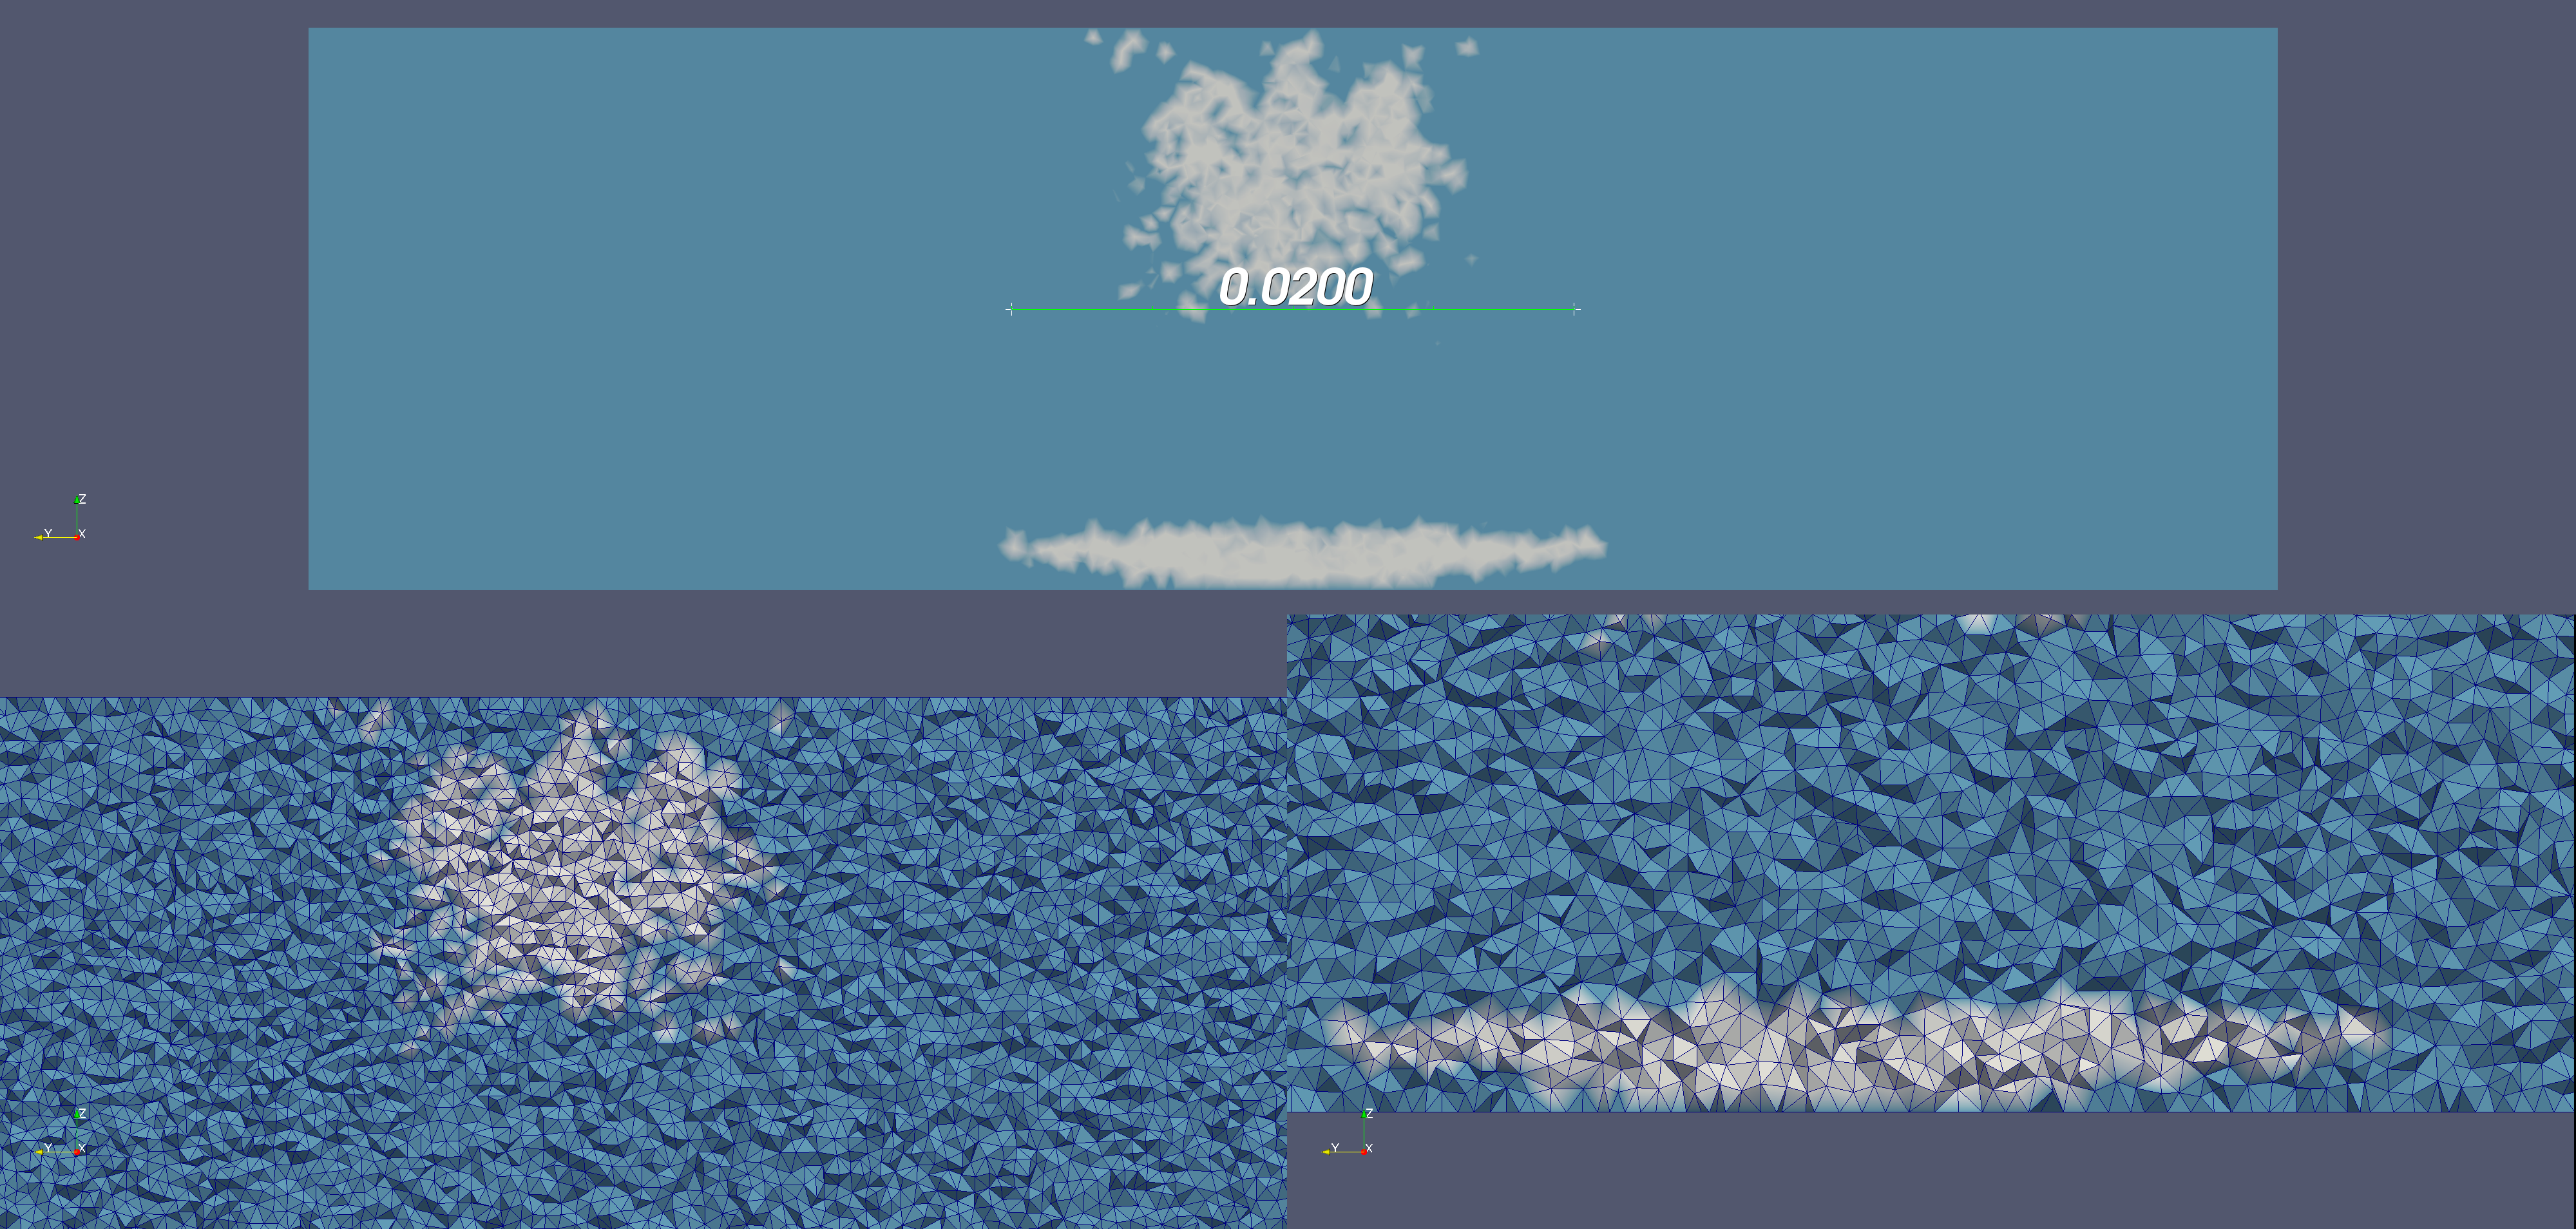
\includegraphics[width=0.9\textwidth]{png/glass/glass-laser-crack-2d.png}
    \end{center}
}

\frame{\frametitle{Стекло: сравнение с~экспериментом}
    \begin{minipage}[h]{0.49\textwidth}
        \begin{center}
            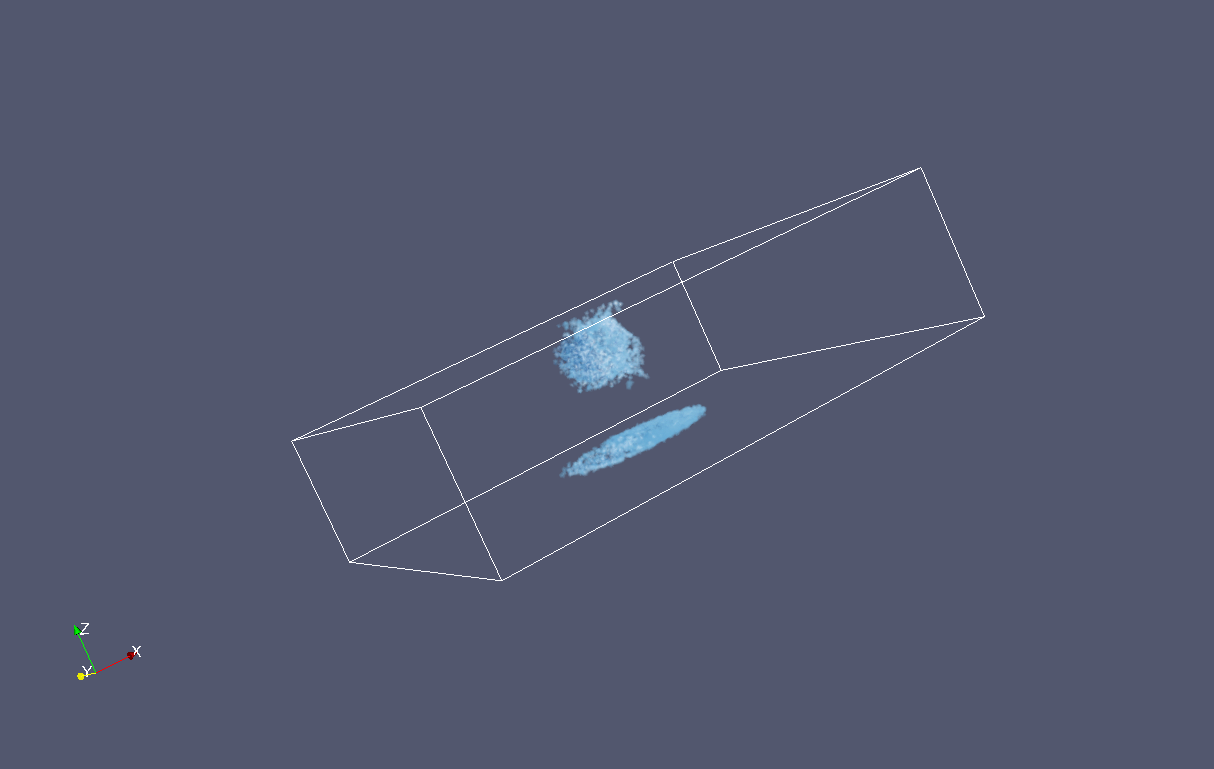
\includegraphics[width=\textwidth]{png/glass/glass-laser-crack-3d.png}
        \end{center}
    \end{minipage}
    \begin{minipage}[h]{0.49\textwidth}
        \begin{center}
            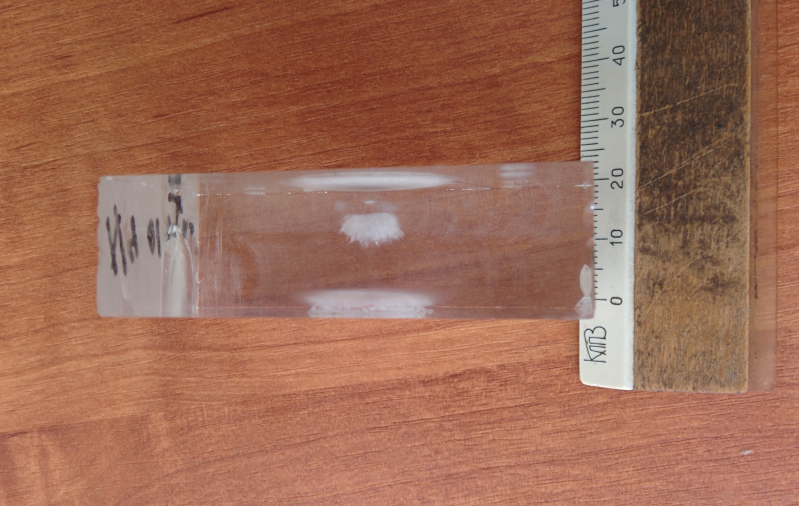
\includegraphics[width=\textwidth]{png/glass/experiment.png}
        \end{center}
    \end{minipage}
}

\frame{\frametitle{Прозрачная броня}
    \begin{minipage}[h!]{0.4\textwidth}
        \begin{center}
            \begin{figure}[h]
                \tikzset{every picture/.style={scale=0.7}}
                \subfile{tikz/armor}
            \end{figure}
        \end{center}
    \end{minipage}
    \qquad{\color{black}\vrule}\qquad
    \begin{minipage}[h!]{0.4\textwidth}
        \small
        \begin{itemize}
            \item Стекло (10~мм)
            \item Клей (2~мм)
            \item Стекло (5~мм)
            \item Клей (2~мм)
            \item Стекло (5~мм)
            \item Клей (2~мм)
            \item Пластик (10~мм)
        \end{itemize}
    \end{minipage}
    \begin{minipage}[h!]{0.4\textwidth}
        \begin{center}
            \textbf{Толщина брони} \\
            \textbf{Радиус шарика} \\
            \textbf{Скорость столкновения}
        \end{center}
    \end{minipage}
    \qquad{\color{black}\vrule}\qquad
    \begin{minipage}[h!]{0.4\textwidth}
        36~мм \\
        5~мм \\
        1000~м/с
    \end{minipage}
}

\begin{python}
#!/bin/env python2
# -*- coding: utf-8 -*-
for n in ["001", "130", "150", "170", "190", "210", "230", "250"]:
    print('\\frame{\\frametitle{Прозрачная броня: разрушение}')
    print('\\begin{center}')
    print('\\includegraphics[width=0.45\\textwidth]{jpg/armor/50/image%s-failed-contact.jpg}' % n)
    print('\\includegraphics[width=0.45\\textwidth]{jpg/armor/50/image%s-crack.jpg}' % n)
    print('\\newline')
    print('\\includegraphics[width=0.45\\textwidth]{jpg/armor/50/image%s-failed-contact-delamination.jpg}' % n)
    print('\\end{center}}')
    print('\\addtocounter{framenumber}{-1}')
\end{python}

\addtocounter{framenumber}{+1}

\frame{\frametitle{Случай орторомбической анизотропии}
    Свойства материала различны по~всем трём направлениям \newline
    \newline
    \begin{minipage}[h!]{0.4\textwidth}
        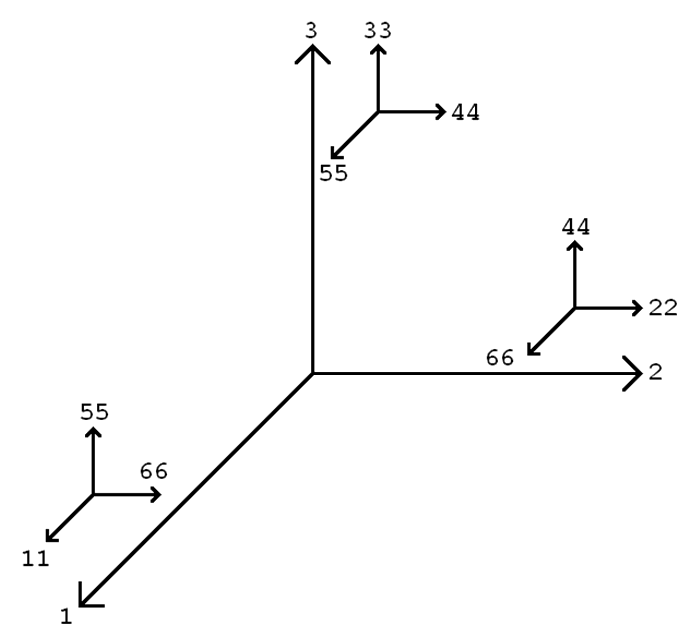
\includegraphics[width=\textwidth]{png/anisotropy/orthorhombic.png}
    \end{minipage}
    \tiny
    \begin{minipage}[h!]{0.5\textwidth}
        \begin{align*}
            c_{ik} =
            \left( \begin{array}{cccccccccccc}
            c_{11} & c_{12} & c_{13} & 0 & 0 & 0 \\
            c_{12} & c_{22} & c_{23} & 0 & 0 & 0 \\
            c_{13} & c_{23} & c_{33} & 0 & 0 & 0 \\
            0 & 0 & 0 & c_{44} & 0 & 0 \\
            0 & 0 & 0 & 0 & c_{55} & 0 \\
            0 & 0 & 0 & 0 & 0 & c_{66}
            \end{array} \right){}
        \end{align*}
    \end{minipage}
    \normalsize
}

\frame{\frametitle{Случай трансверсальной изотропии}
    Существует одно направление, в~котором свойства материала отличаются \newline
    \newline
    \begin{minipage}[h!]{0.4\textwidth}
        \begin{align*}
            \left( \begin{array}{cccccccccccc}
            c_{11} & c_{12} & c_{13} & 0 & 0 & 0 \\
            c_{12} & c_{11} & c_{13} & 0 & 0 & 0 \\
            c_{13} & c_{13} & c_{33} & 0 & 0 & 0 \\
            0 & 0 & 0 & c_{44} & 0 & 0 \\
            0 & 0 & 0 & 0 & c_{44} & 0 \\
            0 & 0 & 0 & 0 & 0 & c_{66}
            \end{array} \right)
        \end{align*}
    \end{minipage}
    \begin{minipage}[h!]{0.3\textwidth}
        $c_{66} = \frac{c_{11} - c_{12}}{2}$
    \end{minipage}
}

\frame{\frametitle{Объёмное разрушение в~композиционном материале}
    \begin{minipage}[h!]{0.20\textwidth}
        \begin{figure}[h]
            \tiny
            \begin{center}
                \tikzset{every picture/.style={scale=0.25}}
                \subfile{tikz/destruction_statement}
            \end{center}
        \end{figure}
    \end{minipage}
    \qquad{\color{black}\vrule}\qquad
    \begin{minipage}[h!]{0.60\textwidth}
        \begin{tabular}[h!]{l|l}
            \textbf{Материал} & Стеклопластик \\
            \textbf{Тип} & Анизотропный \\
            \textbf{Радиус шарика} & 3~см \\
            \textbf{Толщина преграды} & 3~см \\
            \textbf{Скорость соударения} & 90~м/с \\
        \end{tabular}
    \end{minipage}
}

\frame{\frametitle{Объёмное разрушение в~композиционном материале}
    \Wider{
        \centering
        \tiny
        \begin{tabular}{|L{1.6cm}|C{1.5cm}|C{1.5cm}|C{1.5cm}|C{1.5cm}|C{1.5cm}|} \hline
        & Друкер-Прагер & Хашин & Пак & Цай-Хилл & Цай-Ву \\ \hline
        Учёт наличия матрицы и волокон & Нет & Да & Да & Нет & Нет \\ \hline
        Различие пределов на~сжатие и растяжение & Да & Да & Да & Нет & Да \\ \hline
        Различие механизмов разрушения & Нет & Да & Да & Нет & Нет \\ \hline
        Используемая мера разрушения & Скаляр & Скаляр & Вектор & Скаляр & Скаляр \\ \hline
        Отсутствие внутренних параметров модели & Да & Да & Нет & Да & Да \\ \hline
        Целевой материал & Однородный анизотропный материал & Армированный монослой &
                           Армированный монослой & Однородный анизотропный материал &
                           Однородный анизотропный материал \\ \hline
        \end{tabular}
    }
}

\begin{frame}
    \frametitle{Сравнение критериев разрушения}
    \vspace{-2.5em}
    \begin{center}
        \begin{minipage}[h]{0.33\textwidth}
            \begin{figure}[h]
                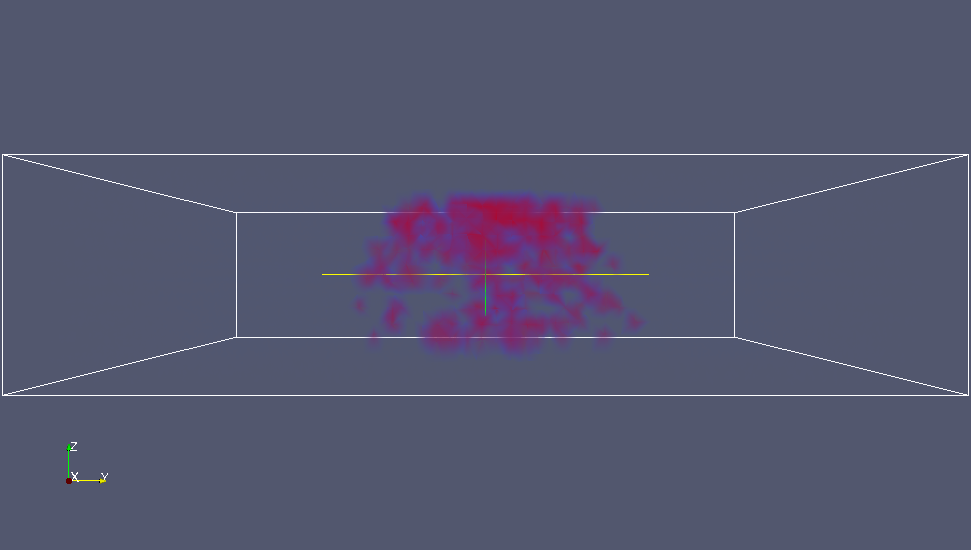
\includegraphics[width=\textwidth]{png/destruction/x-drpr-x-.png}
                \tiny
                \caption{Критерий Друкера-Прагера}
            \end{figure}
        \end{minipage}
        \begin{minipage}[h]{0.33\textwidth}
            \begin{figure}[h]
                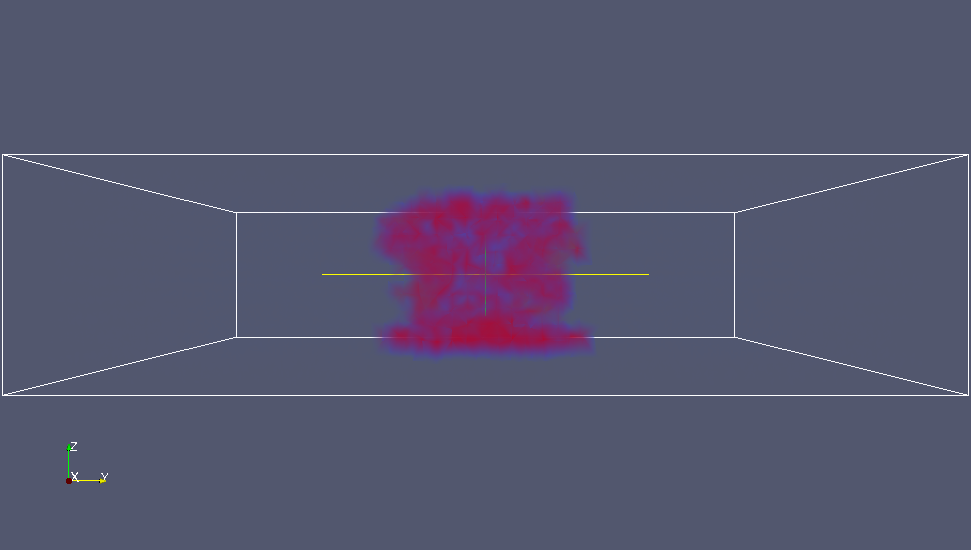
\includegraphics[width=\textwidth]{png/destruction/x-hashin-x-.png}
                \tiny
                \caption{Критерий Хашина}
            \end{figure}
        \end{minipage}
        \begin{minipage}[h]{0.33\textwidth}
            \begin{figure}[h]
                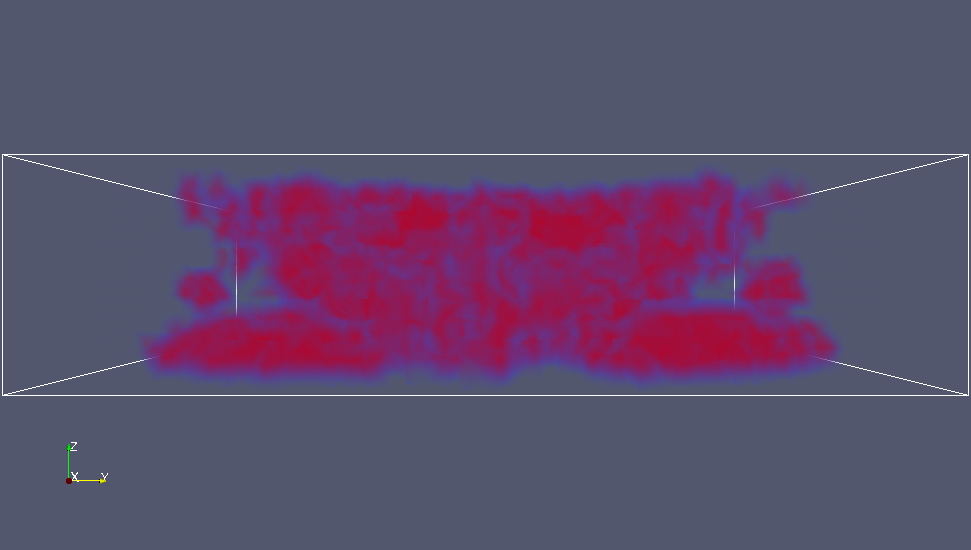
\includegraphics[width=\textwidth]{png/destruction/x-puck-x-.png}
                \tiny
                \caption{Критерий Пака}
            \end{figure}
        \end{minipage}
        \begin{minipage}[h]{0.33\textwidth}
            \begin{figure}[h]
                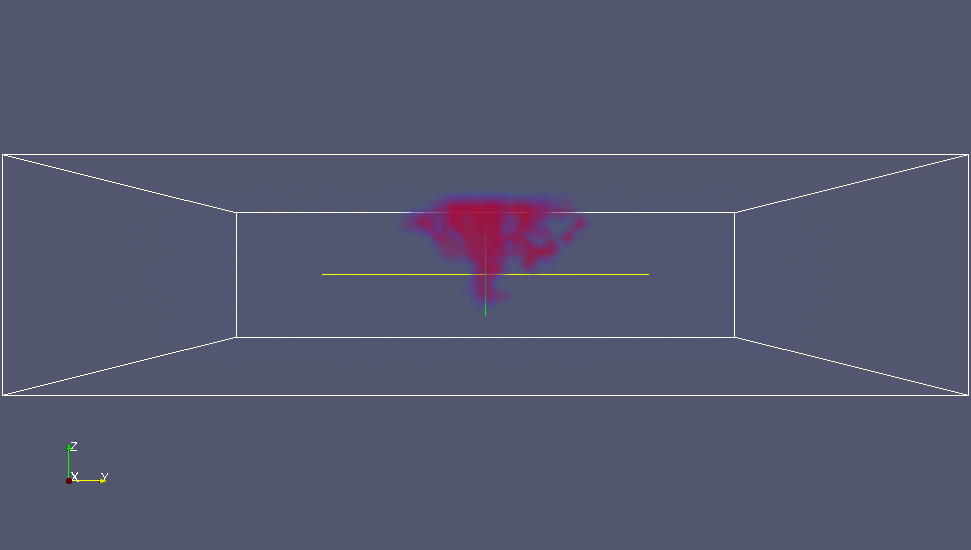
\includegraphics[width=\textwidth]{png/destruction/x-tsaihill-x-.png}
                \tiny
                \caption{Критерий Цая-Хилла}
            \end{figure}
        \end{minipage}
        \begin{minipage}[h]{0.33\textwidth}
            \begin{figure}[h]
                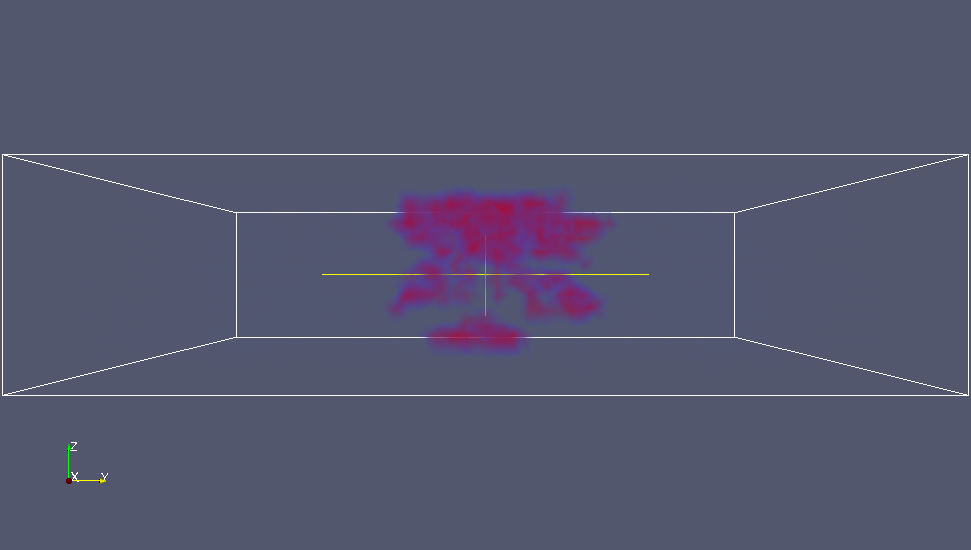
\includegraphics[width=\textwidth]{png/destruction/x-tsaiwu-x-.png}
                \tiny
                \caption{Критерий Цая-Ву}
            \end{figure}
        \end{minipage}
    \end{center}
\end{frame}

\frame{\frametitle{Объёмное разрушение в~композиционном материале}
    \Wider{
        \begin{minipage}[h!]{0.45\textwidth}
            \begin{figure}[h]
                \begin{center}
                    \tikzset{every picture/.style={scale=0.035}}
                    \subfile{tikz/3_stringer_panel}
                \end{center}
            \end{figure}
            \small
            \begin{itemize}
                \item Удар в~обшивку или стрингер
                \item Несколько энергий удара
                \item Различные критерии разрушения
            \end{itemize}
        \end{minipage}
        \begin{minipage}[h!]{0.53\textwidth}
            \begin{center}
                \begin{tabular}{l | l}
                    $E_{11+}$ & 16483 $\textnormal{кгс/мм}^2$ \\
                    $E_{11-}$ & 13376 $\textnormal{кгс/мм}^2$ \\
                    $E_{22+}$ & 805 $\textnormal{кгс/мм}^2$ \\
                    $E_{22-}$ & 854 $\textnormal{кгс/мм}^2$ \\
                    $G_{12}$  & 437 $\textnormal{кгс/мм}^2$ \\
                    $\nu_{12}$ & 0.32 \\
                    $\sigma_{11+}$ & 263 $\textnormal{кгс/мм}^2$ \\
                    $\sigma_{11-}$ & 153 $\textnormal{кгс/мм}^2$ \\
                    $\sigma_{22+}$ & 8.6 $\textnormal{кгс/мм}^2$ \\
                    $\sigma_{22-}$ & 21.3 $\textnormal{кгс/мм}^2$ \\
                    $\tau_{12}$ & 11.2
                \end{tabular}
            \end{center}
        \end{minipage}
    }
}

\frame{\frametitle{Объёмное разрушение в~композиционном материале}
    \begin{figure}[h]
        \begin{center}
            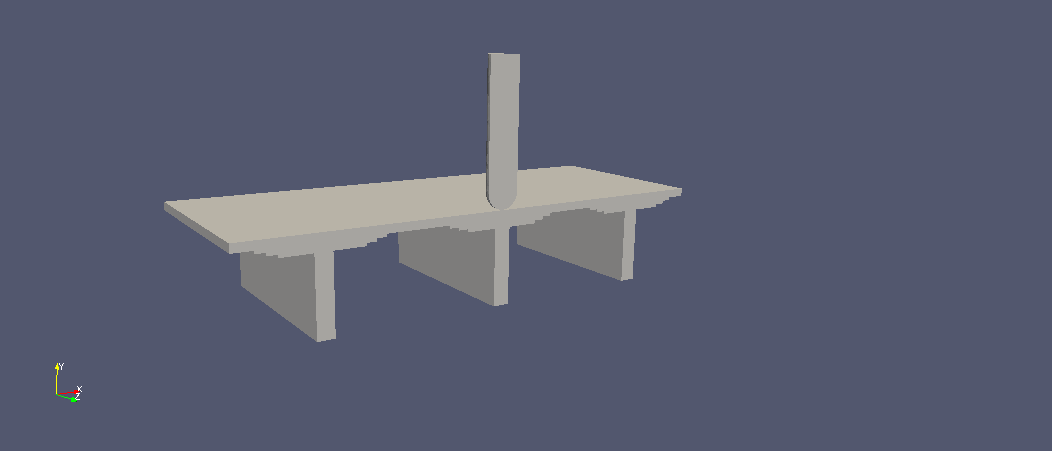
\includegraphics[width=0.7\textwidth]{png/3-stringer-panel/panel-3d-stringer.png}
        \end{center}
    \end{figure}
    \begin{figure}[h]
        \begin{center}
            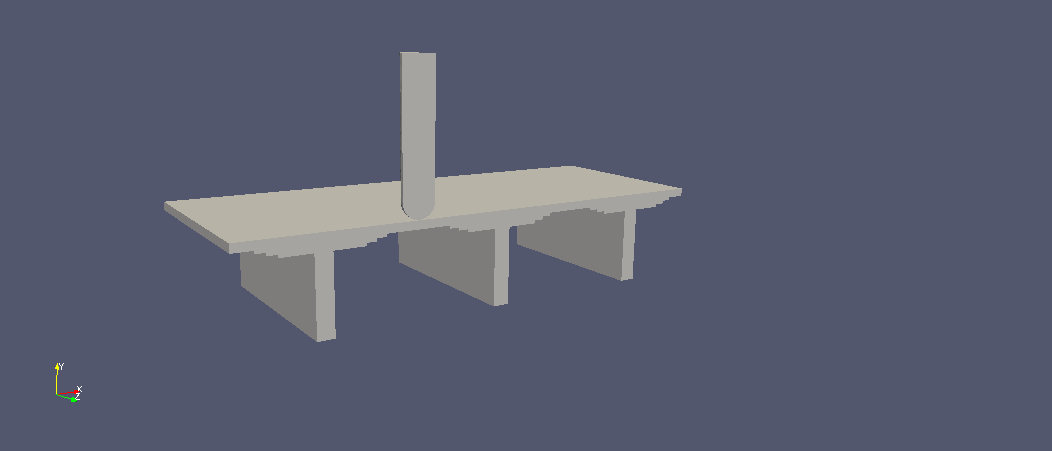
\includegraphics[width=0.7\textwidth]{png/3-stringer-panel/panel-3d-cover.png}
        \end{center}
    \end{figure}
}

\begin{frame}
    \frametitle{Удар в обшивку}
    \begin{center}
        \begin{minipage}[h]{0.30\textwidth}
            \begin{figure}[h]
                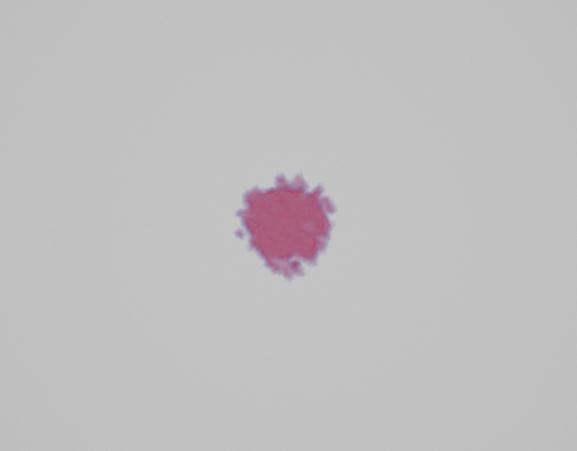
\includegraphics[width=\textwidth]{png/3-stringer-panel/cover-drucker-prager.png}
                \tiny
                \caption{Критерий Друкера-Прагера}
            \end{figure}
        \end{minipage}
        \begin{minipage}[h]{0.30\textwidth}
            \begin{figure}[h]
                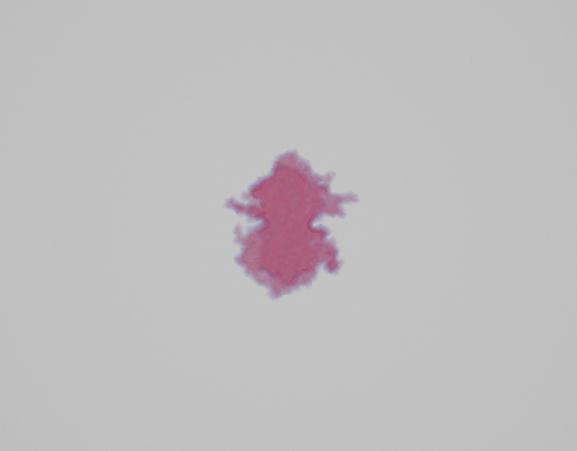
\includegraphics[width=\textwidth]{png/3-stringer-panel/cover-hashin.png}
                \tiny
                \caption{Критерий Хашина}
            \end{figure}
        \end{minipage}
        \begin{minipage}[h]{0.30\textwidth}
            \begin{figure}[h]
                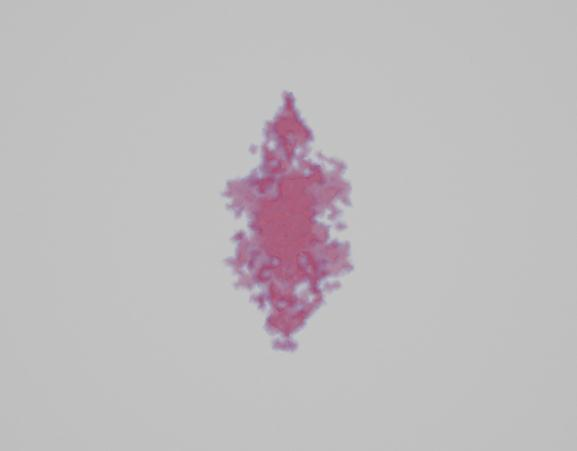
\includegraphics[width=\textwidth]{png/3-stringer-panel/cover-puck.png}
                \tiny
                \caption{Критерий Пака}
            \end{figure}
        \end{minipage}
        \begin{minipage}[h]{0.30\textwidth}
            \begin{figure}[h]
                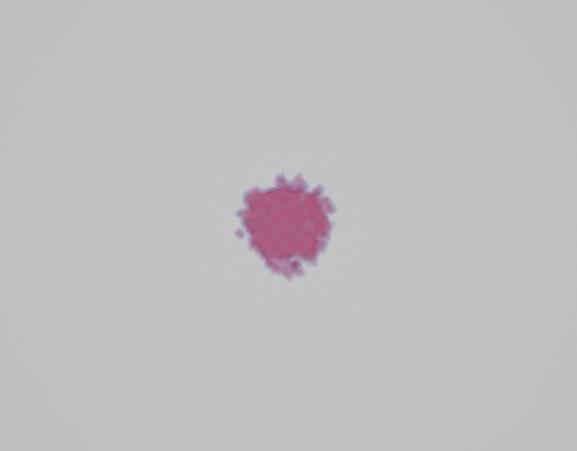
\includegraphics[width=\textwidth]{png/3-stringer-panel/cover-tsai-hill.png}
                \tiny
                \caption{Критерий Цая-Хилла}
            \end{figure}
        \end{minipage}
        \begin{minipage}[h]{0.30\textwidth}
            \begin{figure}[h]
                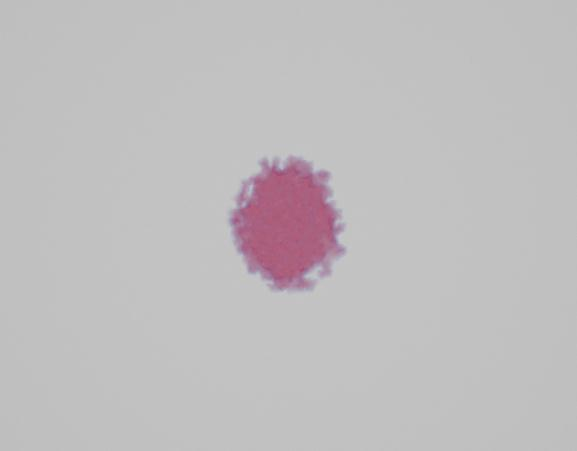
\includegraphics[width=\textwidth]{png/3-stringer-panel/cover-tsai-wu.png}
                \tiny
                \caption{Критерий Цая-Ву}
            \end{figure}
        \end{minipage}
    \end{center}
\end{frame}

\begin{frame}
    \frametitle{Удар в стрингер}
    \begin{center}
        \begin{minipage}[h]{0.30\textwidth}
            \begin{figure}[h]
                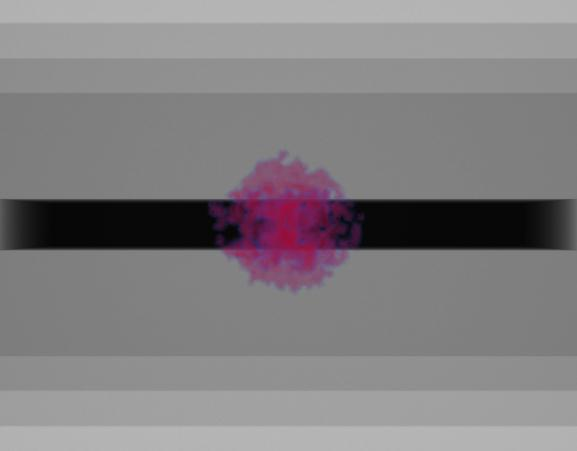
\includegraphics[width=\textwidth]{png/3-stringer-panel/stringer-drucker-prager.png}
                \tiny
                \caption{Критерий Друкера-Прагера}
            \end{figure}
        \end{minipage}
        \begin{minipage}[h]{0.30\textwidth}
            \begin{figure}[h]
                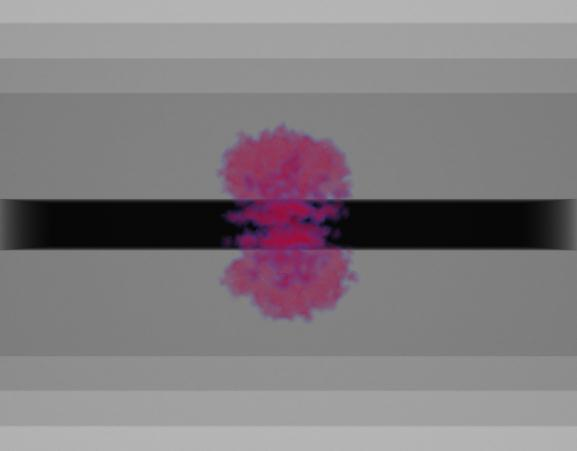
\includegraphics[width=\textwidth]{png/3-stringer-panel/stringer-hashin.png}
                \tiny
                \caption{Критерий Хашина}
            \end{figure}
        \end{minipage}
        \begin{minipage}[h]{0.30\textwidth}
            \begin{figure}[h]
                \includegraphics[width=\textwidth]{png/3-stringer-panel/stringer-puck.png}
                \tiny
                \caption{Критерий Пака}
            \end{figure}
        \end{minipage}
        \begin{minipage}[h]{0.30\textwidth}
            \begin{figure}[h]
                \includegraphics[width=\textwidth]{png/3-stringer-panel/stringer-tsai-hill.png}
                \tiny
                \caption{Критерий Цая-Хилла}
            \end{figure}
        \end{minipage}
        \begin{minipage}[h]{0.30\textwidth}
            \begin{figure}[h]
                \includegraphics[width=\textwidth]{png/3-stringer-panel/stringer-tsai-wu.png}
                \tiny
                \caption{Критерий Цая-Ву}
            \end{figure}
        \end{minipage}
    \end{center}
\end{frame}

\frame{\frametitle{Композиционная панель: результаты}
    \tiny
    \begin{table}[h!]
        \centering
        \begin{tabular}{| L{2.0cm} | C{1.0cm} | C{1.0cm} | C{1.0cm} | C{1.0cm} | C{1.0cm} | C{1.0cm} |}
            \hline
            \multirow{2}{2.0cm}{\textbf{Постановка задачи}} & \multicolumn{6}{ c| } {\textbf{Размер разрушенной области, мм}} \\
            \cline{2-7}
            & \textbf{ДП} & \textbf{Х} & \Good{П} & \textbf{ЦХ} & \textbf{ЦВ} & \textbf{Э} \\
            \hline
            \textbf{Удар в~обшивку, 90 Дж} & 40x40 & 60x45 & 100x52 & 40x40 & 52x44 & 120x65 \\
            \hline
            \textbf{Удар в~стрингер, 135 Дж} & 40x40 & 52x35 & 65x32 & 40x40 & 45x30 & 80x30 \\
            \hline
        \end{tabular}
    \end{table}
    \begin{center}
        \includegraphics[width=0.2\textwidth]{png/3-stringer-panel/experiment-cover.png}
        \qquad\qquad\qquad
        \includegraphics[width=0.2\textwidth]{png/3-stringer-panel/experiment-stringer.png}
    \end{center}
}

\frame{\frametitle{Деламинация в~композиционном материале}
    \Wider{
        \begin{minipage}[h!]{0.6\textwidth}
            \begin{figure}[h]
                \includegraphics[width=\textwidth]{png/destruction/gen-2l.png}
            \end{figure}
        \end{minipage}
        \begin{minipage}[h!]{0.35\textwidth}
            \begin{scriptsize}
                \begin{tabular}{l | l | l}
                          & CFRP & GFRP \\
                    \hline
                    $E_1$ & 135 ГПа & 37.9 ГПа \\
                    $E_2$ & 10 ГПа & 9.67 ГПа \\
                    $E_3$ & 10 ГПа & 9.67 ГПа \\
                    $G_{12}$  & 5.5 ГПа & 3.72 ГПа \\
                    $G_{13}$  & 5.5 ГПа & 3.72 ГПа \\
                    $G_{23}$  & 4.5 ГПа & 3.72 ГПа \\
                    $\nu_{12}$ & 0.0183 & 0.00855 \\
                    $\nu_{13}$ & 0.45 & 0.296 \\
                    $\nu_{23}$ & 0.25 & 0.4 \\
                    $\rho$ & 1489 $\textnormal{кг/м}^3$ & 1620 $\textnormal{кг/м}^3$
                \end{tabular}
            \end{scriptsize}
        \end{minipage}
    }
}

\begin{frame}
    \frametitle{Деламинация в~композиционном материале: CFRP}
    \vspace{-2.5em}
    \begin{center}
        \begin{minipage}[h]{0.33\textwidth}
            \begin{figure}[h]
                \includegraphics[width=\textwidth]{png/destruction/2lc-drpr-delam.png}
                \tiny
                \caption{Критерий Друкера-Прагера}
            \end{figure}
        \end{minipage}
        \begin{minipage}[h]{0.33\textwidth}
            \begin{figure}[h]
                \includegraphics[width=\textwidth]{png/destruction/2lc-hashin-delam.png}
                \tiny
                \caption{Критерий Хашина}
            \end{figure}
        \end{minipage}
        \begin{minipage}[h]{0.33\textwidth}
            \begin{figure}[h]
                \includegraphics[width=\textwidth]{png/destruction/2lc-puck-delam.png}
                \tiny
                \caption{Критерий Пака}
            \end{figure}
        \end{minipage}
        \begin{minipage}[h]{0.33\textwidth}
            \begin{figure}[h]
                \includegraphics[width=\textwidth]{png/destruction/2lc-tsaihill-delam.png}
                \tiny
                \caption{Критерий Цая-Хилла}
            \end{figure}
        \end{minipage}
        \begin{minipage}[h]{0.33\textwidth}
            \begin{figure}[h]
                \includegraphics[width=\textwidth]{png/destruction/2lc-tsaiwu-delam.png}
                \tiny
                \caption{Критерий Цая-Ву}
            \end{figure}
        \end{minipage}
    \end{center}
\end{frame}

\begin{frame}
    \frametitle{Деламинация в~композиционном материале: GFRP}
    \vspace{-2.5em}
    \begin{center}
        \begin{minipage}[h]{0.33\textwidth}
            \begin{figure}[h]
                \includegraphics[width=\textwidth]{png/destruction/2lg-drpr-delam.png}
                \tiny
                \caption{Критерий Друкера-Прагера}
            \end{figure}
        \end{minipage}
        \begin{minipage}[h]{0.33\textwidth}
            \begin{figure}[h]
                \includegraphics[width=\textwidth]{png/destruction/2lg-hashin-delam.png}
                \tiny
                \caption{Критерий Хашина}
            \end{figure}
        \end{minipage}
        \begin{minipage}[h]{0.33\textwidth}
            \begin{figure}[h]
                \includegraphics[width=\textwidth]{png/destruction/2lg-puck-delam.png}
                \tiny
                \caption{Критерий Пака}
            \end{figure}
        \end{minipage}
        \begin{minipage}[h]{0.33\textwidth}
            \begin{figure}[h]
                \includegraphics[width=\textwidth]{png/destruction/2lg-tsaihill-delam.png}
                \tiny
                \caption{Критерий Цая-Хилла}
            \end{figure}
        \end{minipage}
        \begin{minipage}[h]{0.33\textwidth}
            \begin{figure}[h]
                \includegraphics[width=\textwidth]{png/destruction/2lg-tsaiwu-delam.png}
                \tiny
                \caption{Критерий Цая-Ву}
            \end{figure}
        \end{minipage}
    \end{center}
\end{frame}

\frame{\frametitle{Результаты}
    \Wider{
        \begin{small}
            \begin{itemize}
                \item Реализован численный метод для моделирования волновых процессов в~анизотропных средах
                \item Исследован набор критериев разрушения
                \item Реализован и верифицирован комбинированный метод (SPH+GCM)
                \item Метод маркеров адаптирован для использования вместе с~СХМ
                \item Решён ряд практически значимых задач:
                \begin{itemize}
                    \item удар по многослойной стеклянной конструкции
                    \item разрушение стекла под действием ударной нагрузки
                    \item удар по~авиационной композиционной панели
                    \item падение самолёта на крышу здания
                    \item столкновение спутника и микрометеорита
                \end{itemize}
            \end{itemize}
        \end{small}
    }
}

\frame{\frametitle{Публикации}
\tiny
\begin{enumerate}
    \item Беклемышева K. А., Васюков А.В., Ермаков А.С., Петров И. Б.  Численное моделирование волновых процессов в~многослойных материалах при динамическом внешнем воздействии. // Вестник Балтийского федерального университета им. И. Канта.~--- 2013. Вып. 10. С. 7--14.
    \item Васюков А.В., Ермаков А.С., Петров И.Б., Потапов А.П., Фаворская А.В., Шевцов А.В. Комбинирование сеточно-характеристического метода и метода сглаженных частиц в~задачах компьютерного моделирования упругопластических тел // Журнал "Информационные технологии".~--- 2014 г.~--- № 3.~--- С. 19--24.
    \item Петров И. Б., Фаворская А. В., Шевцов А. В., Васюков А. В., Потапов А. П., Ермаков А. С. Сеточно-характеристический комбинированный метод для численного решения динамических пространственных упругопластических задач. // Журнал вычислительной математики и математической физики.~--- 2014.~--- Т. 54.~--- № 7.~--- С. 1203 -- 1217.
    \item Petrov I.B., Favorskaya A. V., Shevtsov A. V., Vasyukov A. V., Potapov A.P., Ermakov A. S. Combined Grid Characteristic Method for the Numerical Solution of Three Dimensional Dynamical Elastoplastic Prob\-lems. // Computational Mathematics and Mathematical Physics. -- 2014.~--- Vol. 54.~--- No. 7~--- pp. 1176 -- 1189
    \item Петров И. Б., Фаворская А. В.,  Васюков А. В., Ермаков А. С., Беклемышева К. А., Казаков А. О., Новиков А. В. О~численном моделировании волновых процессов в~анизотропных средах . // Журнал "Доклады Академии Наук".~--- 2014.~--- Т. 26.~--- № 7.~--- С. 19 -- 32
\end{enumerate}
}
\frame{\frametitle{Публикации}
\tiny
\begin{enumerate}
    \setcounter{enumi}{5}
    \item Петров И. Б., Фаворская А. В., Шевцов А. В., Васюков А. В., Потапов А. П., Ермаков А. С. О~комбинированном методе для численного решения динамических пространственных упругопластических задач. // Журнал "Доклады Академии Наук".~--- 2015.~--- Т. 460.~--- № 4.~--- С. 389--392
    \item Беклемышева K. А., Васюков А.В., Ермаков А.С., Петров И. Б, А.С. Дзюба, В.И. Голован. Численное моделирование динамических процессов при низкоскоростном ударе по~композитной стрингерной панели // Математическое моделирование.~--- 2014.~--- Т. 26, No 9.~--- С. 96--110.
    \item Беклемышева K. А., Васюков А.В., Ермаков А.С., Петров И. Б.  Численное моделирование волновых процессов в~многослойных материалах при динамическом внешнем воздействии. // Труды 55-й научной конференции МФТИ.~--- 2012. Ч. 3. Т. 2. С. 28--29
    \item Ермаков А.С., Васюков А.В. О~построении параллельной версии сеточно-характеристического метода. // Сб. трудов Математические и информационные модели управления, Москва, 2013г., С. 58--64.
    \item Беклемышева K. А., Васюков А.В., Ермаков А.С.  Численное моделирование деформации полимерного композитного материала при сжатии. // М.:МФТИ, Сб. трудов МФТИ: Математические и информационные модели управления.~--- 2013.
    \item Беклемышева K. А., Васюков А.В., Ермаков А.С., Петров И. Б. Численное моделирование разрушения конструкций из~многослойных материалов при низкоскоростном соударении. // Труды 56-й научной конференции МФТИ.~--- 2013. Ч. 3. Т. 2. С. 25--26
\end{enumerate}
}

\plain{Спасибо за~внимание}

\end{document}
